\chapter{Introduction}
\label{chap:introduction}

%\itquote{
%Enjoyment appears at the boundary between boredom and anxiety,
%when the challenges are just balanced with the person's capacity to act.
%}{Mihaly Csikszentmihalyi}

\itquote{
To prepare humanity for the next 100 years, we need more of our children to learn computer programming skills, regardless of their future profession. Along with reading and writing, the ability to program is going to define what an educated person is.}
{S. Khan}

Artificial intelligence proved to be a powerful tool for tackling difficult problems,
from playing chess to driving autonomous cars. % TODO: references
Can we use the artificial intelligence to optimize optimize learning of programming?
%This thesis explores how we can use artificial intelligence to optimize
%learning of introductory programming.
%This thesis explores how can be artificial intelligence used to optimize
%learning of introductory programming.
Adaptive learning systems have been already successfully used in many domains
\cite{alg.evaluation-geography,
matmat.response-times, mathsgarden, sqltutor}.
% maths += Cognitive Tutor (?mastery-learning-scale), ASSiSTments (Koedinger
% 2010), ALEKS
% TODO: the last 3 are all maths -> find another domain
Nevertheless, the most popular introductory programming tutorials,
Hours of Code \cite{hour-of-code},
offer the same fixed sequence of tasks for everybody,
leading to a suboptimal experience.
Artificial intelligence can be used to personalize the sequence of tasks.
% for each student.
By giving students tasks of difficulty matching their skill,
%neither too easy, nor too difficult,
we help them to achieve complete immersion into the problem solving
activity (figure \ref{fig:flow}).
This \emph{state of flow} \cite{flow}
is essential for the optimal learning experience
\cite{adaptive-practice}.

\begin{figure}[htb]
  \centering
  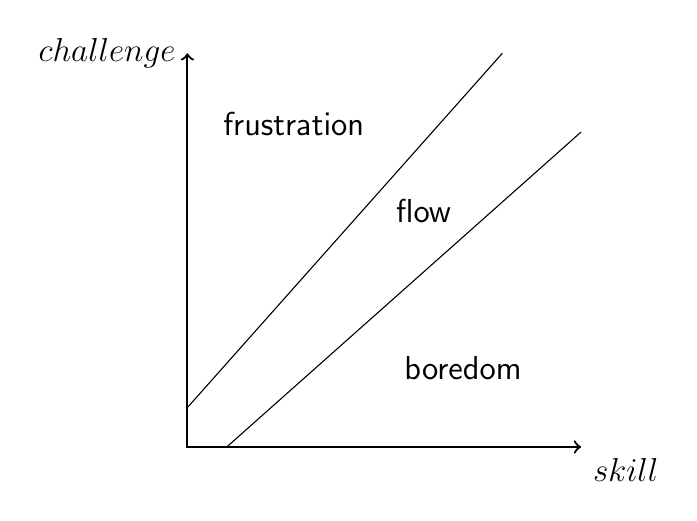
\begin{tikzpicture}[font=\sffamily,xscale=5, yscale=5]
  \large
  %\draw [lightgray, fill=gray] (0,0) -- (0.1,0) -- (1,0.8) -- (0.8,1) -- (0,0.1) -- (0,0);
  \draw (0.1,0) -- (1,0.8);
  \draw (0,0.1) -- (0.8,1);
  \draw [thick, <->] (0,1) node [left] {$challenge$} -- (0,0) -- (1,0) node [below right] {$skill$};
  \node at (0.27,0.82) {frustration};
  \node at (0.6,0.6) {flow};
  \node at (0.7,0.2) {boredom};
  \end{tikzpicture}
  \caption{Relationship between challenge and skill.}
  \label{fig:flow}
\end{figure}

%TODO: related areas
%- introductory programming learning
%- adaptive learning / intelligent tutoring systems
%- recommendation systems (with performance instead of ratings)
%- HCI, (software learnability)
%- games design \cite{book-of-lenses}

How to design a programming game that supports both learning and motivation?
How to model the domain and students of introductory programming?
% OR: How to estimate skills of the students and how to model learning of IP?
Which algorithms to use for task recommendation and mastery learning?
How to evaluate and iteratively improve components of the adaptive learning system?
%How to evaluate if the adaptivity of the system helps to improve learning and engagement?
% TODO: Make sure these questions are answered in the text (or remove them).
To answer these questions, we not only look at the existing systems
and research, but we also develop our own adaptive learning system for
introductory programming, RoboMission\footnote{Available at \url{en.robomise.cz}}
(figure \ref{fig:robomission-task1}).
Development of this system helps us to better understand related challenges
and allow us to collect data that we need to support or reject our hypotheses.
% TODO: And are there such hypotheses in the thesis?
% NOTE: RoboMission = app for efficient and engaging learning of introductory
% programming for children (= mission)

% TODO: English screenshot.
\imgW[0.9]{robomission-task1}%
  {RoboMission is a web application for learning introductory programming %
   using space themed grid world and block-based programming.}

We first look at how the introductory programming is taught
in existing online learning systems
(chapter \ref{chap:learning-programming}),
and describe relevant techniques of adaptive learning
(chapter \ref{chap:adaptive-learning}).
%We focus on models of domain and student for introductory programming,
%algorithms for task recommendation and mastery learning,
%and evaluation of the system and its components.
Then we present a new game designed for learning introductory programming
(chapter \ref{chap:design-of-game}),
approach to adaptivity in our system (chapter \ref{chap:design-of-adaptivity}),
and its implementation (chapter \ref{chap:implementation-of-robomission}).
We conclude the thesis with analyses of collected data
(chapter \ref{chap:analysis}).
